%\renewcommand{\theequation}{\theenumi}
%\begin{enumerate}[label=\arabic*.,ref=\theenumi]
\begin{enumerate}[label=\thesection.\arabic*.,ref=\thesection.\theenumi]
\numberwithin{equation}{enumi}
\item Suppose the equations $AB, BC$ and $CA$ are respectively given by 
		\begin{align}
			\label{eq:tri-sides}
			\vec{n}_i^{\top}\vec{x}=c_i \quad i = 1, 2, 3 
		\end{align}
		The equations of the respective angle bisectors are then given by 
		\begin{align}
			\frac{\vec{n}_i^{\top}\vec{x}-c_i}{\norm{\vec{n}_i}}
		=
	\pm	\frac{\vec{n}_j^{\top}\vec{x}-c_j}{\norm{\vec{n}_j}}
\quad i \ne j
		\end{align}
		Substitute numerical values and find the equations of the angle bisectors of $A, B$ and $C$.
	\\
		%\textbf{Solution :}
	The parametric equations of sides;
	\begin{align}
	BC:\quad &\myvec{11&1}\vec{x}=-38,\\
	CA:\quad &\myvec{1&-1}\vec{x}=2,\\
	AB:\quad &\myvec{7&5}\vec{x}=2\\	  
	\end{align}
	Using the formula mentioned in the question to find out the angular bisector for sides \text{AB} and \text{AC}, naming the angular bisector $L$ we get,
	\begin{align}
		\frac{\vec{n}_{3}^{\top} \vec{x}-c_{3}}{\norm{\vec{n}_{3}}}=\pm \frac{\vec{n}_{2}^{\top} \vec{x}-c_{2}}{\norm{\vec{n}_{2}}}
	\end{align}
	\begin{figure}
	\centering
	\includegraphics[width=\columnwidth]{solutions/1/5/1/figs/angular_bisector.png}
	\caption{Triangle generated using python}
	\label{fig:angular_bisector}
	\end{figure}
	As we can see we will get 2 solutions for $L$. This is because one of them is internal angular bisector and the other is the external angular bisector. Internal angular bisector can be evaluated if we take + in the above formula.
	Hence, $L$ is given by,
	\begin{align}
		\frac{\vec{n}_{3}^{\top} \vec{x}-c_{3}}{\norm{\vec{n}_{3}}}&=\frac{\vec{n}_{2}^{\top} \vec{x}-c_{2}}{\norm{\vec{n}_{2}}}\\
		\implies \brak{\frac{\vec{n_{3}}}{\norm{\vec{n_{3}}}}-\frac{\vec{n_{3}}}{\norm{\vec{n_{3}}}}} \vec{x}&=\brak{\frac{c_{3}}{\norm{\vec{n_{3}}}}-\frac{c_{2}}{\norm{\vec{n_{2}}}}}\\
		\implies \brak{\frac{\myvec{7&5}}{\sqrt{74}}-\frac{\myvec{1&-1}}{\sqrt{2}}} \vec{x}&=\frac{2}{\sqrt{74}}-\frac{2}{\sqrt{2}}\\
		\implies \myvec{\frac{7-\sqrt{37}}{\sqrt{74}}&\frac{5+\sqrt{37}}{\sqrt{74}}}\vec{x}&=\frac{2-2\sqrt{37}}{\sqrt{74}}
	\end{align}
	Hence, the internal angluar bisector of angle $A$, $L$ will be,
	\begin{align}
		\implies\myvec{\frac{7-\sqrt{37}}{\sqrt{74}}&\frac{5+\sqrt{37}}{\sqrt{74}}} \vec{x}=\frac{2-2\sqrt{37}}{\sqrt{74}}
		\label{eq:1.5.1}
	\end{align}
	

  \solution 
The above formula can 
be transformed to the normal equation of angle bisectors as  
\begin{align}
       \myvec{\frac{\vec{n}_i}{\norm{\vec{n}_i}} - \frac{\vec{n}_j}{\norm{\vec{n}_j}}}^{\top}\vec{x}
       =
       \frac{c_i}{\norm{\vec{n}_i}}-\frac{c_j}{\norm{\vec{n}_j}}
\end{align}
\begin{enumerate}
\item From 
		\eqref{eq:geo-norm-vec-ab}
		and 
		\eqref{eq:geo-norm-vec-ca}
the angle Bisector of $A$ is 
\begin{align}
\myvec{
\frac{7}{\sqrt{74}}-\frac{1}{\sqrt{2}} & \frac{5}{\sqrt{74}}+\frac{1}{\sqrt{2}}\\
}
\vec{x}
=\frac{2}{\sqrt{74}}-\frac{2}{\sqrt{2}}
\end{align}
\item Similarly, the angle bisector of $B$ is 
\begin{align}
\myvec{
\frac{11}{\sqrt{122}}+\frac{7}{\sqrt{74}} & \frac{1}{\sqrt{122}}+\frac{5}{\sqrt{74}}\\
}
\vec{x}
=\frac{2}{\sqrt{74}}-\frac{38}{\sqrt{122}}
\end{align}
\item and the angle bisector of $C$ is 
\begin{align}
\myvec{
\frac{11}{\sqrt{122}}+\frac{1}{\sqrt{2}} & \frac{1}{\sqrt{122}}-\frac{1}{\sqrt{2}}\\
}
\vec{x}
=\frac{2}{\sqrt{2}}-\frac{38}{\sqrt{122}}
\end{align}
\end{enumerate}

	\item Find the intersection $\vec{I}$ of the angle bisectors of $B$ and $C$.
	\item Using 
    \eqref{eq:angle2d}
verify that 
		\begin{align}
			\angle BAI = \angle CAI.
		\end{align}
	\item Find the distance from $\vec{I}$ to $BC$.  
  \\
		\solution
Considering
\begin{align}
	BC: \quad \vec{n} ^\top \vec{x} &= c, 
\end{align}
the distance from $\vec{I}$ to $BC$ is 
\begin{align}
\frac{\abs{\vec{n}^\top \vec{I} - c}}{\norm{\vec{n}}} 
\end{align}

 
	\item Repeat the above exercise for the sides $AB$ and $AC$.
	This distance is known as the {\em inradius} $r$.
	\item Draw a circle with center $\vec{I}$ and radius $r$.  $\vec{I}$ is known as the {\em incentre}.
	\item The equation of the {\em incircle} is given by 
		\begin{align}
			\label{eq:incircle}
			\norm{\vec{x}-\vec{I}}^2 = r^2
		\end{align}
		Using the parameteric equation of $BC$, verify that $BC$ intersects the incircle at exactly one point. $BC$ is defined to be a {\em tangent} to the incircle.
		\\
		\iffalse
\let\negmedspace\undefined
\let\negthickspace\undefined
\documentclass[journal,12pt,twocolumn]{IEEEtran}
\usepackage{cite}
\usepackage{amsmath,amssymb,amsfonts,amsthm}
\usepackage{algorithmic}
\usepackage{graphicx}
\usepackage{textcomp}
\usepackage{xcolor}
\usepackage{txfonts}
\usepackage{listings}
\usepackage{enumitem}
\usepackage{mathtools}
\usepackage{gensymb}
\usepackage[breaklinks=true]{hyperref}
\usepackage{tkz-euclide} % loads  TikZ and tkz-base
\usepackage{listings}
\usepackage{gvv}
%
%\usepackage{setspace}
%\usepackage{gensymb}
%\doublespacing
%\singlespacing

%\usepackage{graphicx}
%\usepackage{amssymb}
%\usepackage{relsize}
%\usepackage[cmex10]{amsmath}
%\usepackage{amsthm}
%\interdisplaylinepenalty=2500
%\savesymbol{iint}
%\usepackage{txfonts}
%\restoresymbol{TXF}{iint}
%\usepackage{wasysym}
%\usepackage{amsthm}
%\usepackage{iithtlc}
%\usepackage{mathrsfs}
%\usepackage{txfonts}
%\usepackage{stfloats}
%\usepackage{bm}
%\usepackage{cite}
%\usepackage{cases}
%\usepackage{subfig}
%\usepackage{xtab}
%\usepackage{longtable}
%\usepackage{multirow}
%\usepackage{algorithm}
%\usepackage{algpseudocode}
%\usepackage{enumitem}
%\usepackage{mathtools}
%\usepackage{tikz}
%\usepackage{circuitikz}
%\usepackage{verbatim}
%\usepackage{tfrupee}
%\usepackage{stmaryrd}
%\usetkzobj{all}
%    \usepackage{color}                                            %%
%    \usepackage{array}                                            %%
%    \usepackage{longtable}                                        %%
%    \usepackage{calc}                                             %%
%    \usepackage{multirow}                                         %%
%    \usepackage{hhline}                                           %%
%    \usepackage{ifthen}                                           %%
  %optionally (for landscape tables embedded in another document): %%
%    \usepackage{lscape}     
%\usepackage{multicol}
%\usepackage{chngcntr}
%\usepackage{enumerate}

%\usepackage{wasysym}
%\documentclass[conference]{IEEEtran}
%\IEEEoverridecommandlockouts
% The preceding line is only needed to identify funding in the first footnote. If that is unneeded, please comment it out.

\newtheorem{theorem}{Theorem}[section]
\newtheorem{problem}{Problem}
\newtheorem{proposition}{Proposition}[section]
\newtheorem{lemma}{Lemma}[section]
\newtheorem{corollary}[theorem]{Corollary}
\newtheorem{example}{Example}[section]
\newtheorem{definition}[problem]{Definition}
%\newtheorem{thm}{Theorem}[section] 
%\newtheorem{defn}[thm]{Definition}
%\newtheorem{algorithm}{Algorithm}[section]
%\newtheorem{cor}{Corollary}
\newcommand{\BEQA}{\begin{eqnarray}}
\newcommand{\EEQA}{\end{eqnarray}}
\newcommand{\define}{\stackrel{\triangle}{=}}
\theoremstyle{remark}
\newtheorem{rem}{Remark}

%\bibliographystyle{ieeetr}
\begin{document}
%

\bibliographystyle{IEEEtran}


\vspace{3cm}

\title{
Question 1.5.7
}
\author{ SREEKAR CHEELA - EE22BTECH11051$^{*}$% <-this % stops a space
	\thanks{*The author is with the Department
		of Electrical Engineering, Indian Institute of Technology, Hyderabad
		502285 India e-mail:  ee22btech11051@iith.ac.in. All content in this manual is released under GNU GPL.  Free and open source.}
	
}	
% make the title area
\maketitle

\newpage

\bigskip

\renewcommand{\thefigure}{\theenumi}
\renewcommand{\thetable}{\theenumi}
%\renewcommand{\theequation}{\theenumi}

%\tableofcontents

% Within an equation environment

\textbf{Question :} Draw a circle with its centre as I (incentre) and radius r (inradius)\\
\fi
\textbf{Solution :}
The vertices of the given triangle are:

\begin{align}
	\vec {A}= &\myvec{1\\-1};\\ \vec {B}= &\myvec{-4\\6};\\ \vec {C}= &\myvec{-3\\-5}
\end{align}

The incentre of the triangle is:

	\begin{align}
	\vec{I}=&\myvec{
		-1.48 \\
		-0.79}
	\end{align}

	The inradius of the triangle is:

    \begin{align}
    r = \frac{185+41\sqrt{37}-37\sqrt{61}-\sqrt{2257}}{6\sqrt{74}} = 1.896\\
    \end{align}
\begin{figure}
	\centering
	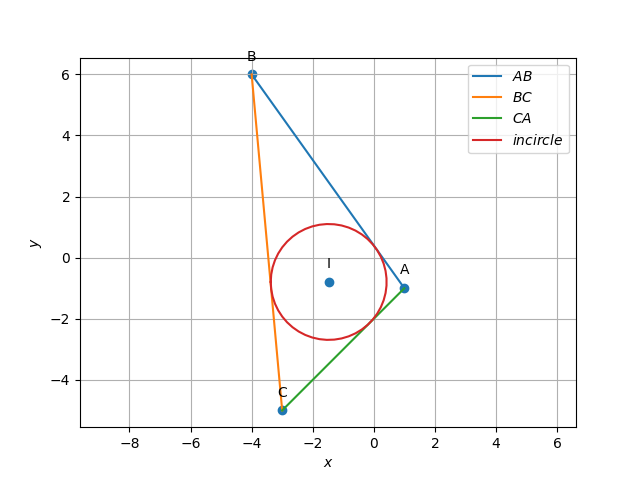
\includegraphics[width=\columnwidth]{solutions/1/5/7/figs/Diagram.png}
	\caption{Triangle with the incircle generated using python}
	\label{fig:Incircle}
\end{figure}

	The equation of the incircle is given as :

	\begin{align}
			\norm{\vec{x}-\vec{I}}^2 = r^2
	\end{align}

	\item Find the {\em point of contact} $\vec{D}_3$ where $BC$ touches the incircle.
		\\
		\solution
Since
	\eqref{eq:incircle-disc}
	has only one root, 
\begin{align}
k=-\frac{\vec{m}^{\top}\brak{\vec{B}-\vec{I}}}{{\ \norm{\vec{m}}^2}}
\end{align}
Substituing the above in 
\eqref{eq:8},
\begin{align}
	\vec{D_{3}} = \vec{B} -\frac{\vec{m}^{\top}\brak{\vec{B}-\vec{I}}}{{\ \norm{\vec{m}}^2}} \vec{m}
\end{align}



  \item Find the other points of contact $\vec{E}_3$ and $\vec{F}_3$.
  \\
		\iffalse
\let\negmedspace\undefined
\let\negthickspace\undefined
\documentclass[journal,12pt,twocolumn]{IEEEtran}
\usepackage{cite}
\usepackage{amsmath,amssymb,amsfonts,amsthm}
\usepackage{algorithmic}
\usepackage{graphicx}
\usepackage{textcomp}
\usepackage{xcolor}
\usepackage{txfonts}
\usepackage{listings}
\usepackage{enumitem}
\usepackage{mathtools}
\usepackage{gensymb}
\usepackage[breaklinks=true]{hyperref}
\usepackage{tkz-euclide} % loads  TikZ and tkz-base
\usepackage{listings}
\usepackage{gvv}
%
%\usepackage{setspace}
%\usepackage{gensymb}
%\doublespacing
%\singlespacing

%\usepackage{graphicx}
%\usepackage{amssymb}
%\usepackage{relsize}
%\usepackage[cmex10]{amsmath}
%\usepackage{amsthm}
%\interdisplaylinepenalty=2500
%\savesymbol{iint}
%\usepackage{txfonts}
%\restoresymbol{TXF}{iint}
%\usepackage{wasysym}
%\usepackage{amsthm}
%\usepackage{iithtlc}
%\usepackage{mathrsfs}
%\usepackage{txfonts}
%\usepackage{stfloats}
%\usepackage{bm}
%\usepackage{cite}
%\usepackage{cases}
%\usepackage{subfig}
%\usepackage{xtab}
%\usepackage{longtable}
%\usepackage{multirow}
%\usepackage{algorithm}
%\usepackage{algpseudocode}
%\usepackage{enumitem}
%\usepackage{mathtools}
%\usepackage{tikz}
%\usepackage{circuitikz}
%\usepackage{verbatim}
%\usepackage{tfrupee}
%\usepackage{stmaryrd}
%\usetkzobj{all}
%    \usepackage{color}                                            %%
%    \usepackage{array}                                            %%
%    \usepackage{longtable}                                        %%
%    \usepackage{calc}                                             %%
%    \usepackage{multirow}                                         %%
%    \usepackage{hhline}                                           %%
%    \usepackage{ifthen}                                           %%
  %optionally (for landscape tables embedded in another document): %%
%    \usepackage{lscape}     
%\usepackage{multicol}
%\usepackage{chngcntr}
%\usepackage{enumerate}

%\usepackage{wasysym}
%\documentclass[conference]{IEEEtran}
%\IEEEoverridecommandlockouts
% The preceding line is only needed to identify funding in the first footnote. If that is unneeded, please comment it out.

\newtheorem{theorem}{Theorem}[section]
\newtheorem{problem}{Problem}
\newtheorem{proposition}{Proposition}[section]
\newtheorem{lemma}{Lemma}[section]
\newtheorem{corollary}[theorem]{Corollary}
\newtheorem{example}{Example}[section]
\newtheorem{definition}[problem]{Definition}
%\newtheorem{thm}{Theorem}[section] 
%\newtheorem{defn}[thm]{Definition}
%\newtheorem{algorithm}{Algorithm}[section]
%\newtheorem{cor}{Corollary}
\newcommand{\BEQA}{\begin{eqnarray}}
\newcommand{\EEQA}{\end{eqnarray}}
\newcommand{\define}{\stackrel{\triangle}{=}}
\theoremstyle{remark}
\newtheorem{rem}{Remark}

%\bibliographystyle{ieeetr}
\begin{document}
%

\bibliographystyle{IEEEtran}


\vspace{3cm}

\title{
Question 1.5.7
}
\author{ SREEKAR CHEELA - EE22BTECH11051$^{*}$% <-this % stops a space
	\thanks{*The author is with the Department
		of Electrical Engineering, Indian Institute of Technology, Hyderabad
		502285 India e-mail:  ee22btech11051@iith.ac.in. All content in this manual is released under GNU GPL.  Free and open source.}
	
}	
% make the title area
\maketitle

\newpage

\bigskip

\renewcommand{\thefigure}{\theenumi}
\renewcommand{\thetable}{\theenumi}
%\renewcommand{\theequation}{\theenumi}

%\tableofcontents

% Within an equation environment

\textbf{Question :} Draw a circle with its centre as I (incentre) and radius r (inradius)\\
\fi
\textbf{Solution :}
The vertices of the given triangle are:

\begin{align}
	\vec {A}= &\myvec{1\\-1};\\ \vec {B}= &\myvec{-4\\6};\\ \vec {C}= &\myvec{-3\\-5}
\end{align}

The incentre of the triangle is:

	\begin{align}
	\vec{I}=&\myvec{
		-1.48 \\
		-0.79}
	\end{align}

	The inradius of the triangle is:

    \begin{align}
    r = \frac{185+41\sqrt{37}-37\sqrt{61}-\sqrt{2257}}{6\sqrt{74}} = 1.896\\
    \end{align}
\begin{figure}
	\centering
	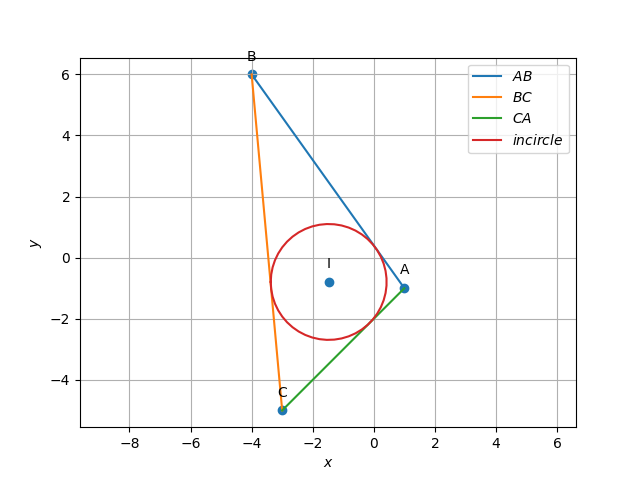
\includegraphics[width=\columnwidth]{solutions/1/5/7/figs/Diagram.png}
	\caption{Triangle with the incircle generated using python}
	\label{fig:Incircle}
\end{figure}

	The equation of the incircle is given as :

	\begin{align}
			\norm{\vec{x}-\vec{I}}^2 = r^2
	\end{align}

	\item Verify that 
		\begin{align}
			AE_3 = AF_3=m, BD_3 = BF_3=n, CD_3 = CE_3=p.
		\end{align}
  \\	\iffalse
\let\negmedspace\undefined
\let\negthickspace\undefined
\documentclass[journal,12pt,twocolumn]{IEEEtran}
\usepackage{cite}
\usepackage{amsmath,amssymb,amsfonts,amsthm}
\usepackage{algorithmic}
\usepackage{graphicx}
\usepackage{textcomp}
\usepackage{xcolor}
\usepackage{txfonts}
\usepackage{listings}
\usepackage{enumitem}
\usepackage{mathtools}
\usepackage{gensymb}
\usepackage[breaklinks=true]{hyperref}
\usepackage{tkz-euclide} % loads  TikZ and tkz-base
\usepackage{listings}
\usepackage{gvv}
%
%\usepackage{setspace}
%\usepackage{gensymb}
%\doublespacing
%\singlespacing

%\usepackage{graphicx}
%\usepackage{amssymb}
%\usepackage{relsize}
%\usepackage[cmex10]{amsmath}
%\usepackage{amsthm}
%\interdisplaylinepenalty=2500
%\savesymbol{iint}
%\usepackage{txfonts}
%\restoresymbol{TXF}{iint}
%\usepackage{wasysym}
%\usepackage{amsthm}
%\usepackage{iithtlc}
%\usepackage{mathrsfs}
%\usepackage{txfonts}
%\usepackage{stfloats}
%\usepackage{bm}
%\usepackage{cite}
%\usepackage{cases}
%\usepackage{subfig}
%\usepackage{xtab}
%\usepackage{longtable}
%\usepackage{multirow}
%\usepackage{algorithm}
%\usepackage{algpseudocode}
%\usepackage{enumitem}
%\usepackage{mathtools}
%\usepackage{tikz}
%\usepackage{circuitikz}
%\usepackage{verbatim}
%\usepackage{tfrupee}
%\usepackage{stmaryrd}
%\usetkzobj{all}
%    \usepackage{color}                                            %%
%    \usepackage{array}                                            %%
%    \usepackage{longtable}                                        %%
%    \usepackage{calc}                                             %%
%    \usepackage{multirow}                                         %%
%    \usepackage{hhline}                                           %%
%    \usepackage{ifthen}                                           %%
  %optionally (for landscape tables embedded in another document): %%
%    \usepackage{lscape}     
%\usepackage{multicol}
%\usepackage{chngcntr}
%\usepackage{enumerate}

%\usepackage{wasysym}
%\documentclass[conference]{IEEEtran}
%\IEEEoverridecommandlockouts
% The preceding line is only needed to identify funding in the first footnote. If that is unneeded, please comment it out.

\newtheorem{theorem}{Theorem}[section]
\newtheorem{problem}{Problem}
\newtheorem{proposition}{Proposition}[section]
\newtheorem{lemma}{Lemma}[section]
\newtheorem{corollary}[theorem]{Corollary}
\newtheorem{example}{Example}[section]
\newtheorem{definition}[problem]{Definition}
%\newtheorem{thm}{Theorem}[section] 
%\newtheorem{defn}[thm]{Definition}
%\newtheorem{algorithm}{Algorithm}[section]
%\newtheorem{cor}{Corollary}
\newcommand{\BEQA}{\begin{eqnarray}}
\newcommand{\EEQA}{\end{eqnarray}}
\newcommand{\define}{\stackrel{\triangle}{=}}
\theoremstyle{remark}
\newtheorem{rem}{Remark}

%\bibliographystyle{ieeetr}
\begin{document}
%

\bibliographystyle{IEEEtran}


\vspace{3cm}

\title{
Question 1.5.7
}
\author{ SREEKAR CHEELA - EE22BTECH11051$^{*}$% <-this % stops a space
	\thanks{*The author is with the Department
		of Electrical Engineering, Indian Institute of Technology, Hyderabad
		502285 India e-mail:  ee22btech11051@iith.ac.in. All content in this manual is released under GNU GPL.  Free and open source.}
	
}	
% make the title area
\maketitle

\newpage

\bigskip

\renewcommand{\thefigure}{\theenumi}
\renewcommand{\thetable}{\theenumi}
%\renewcommand{\theequation}{\theenumi}

%\tableofcontents

% Within an equation environment

\textbf{Question :} Draw a circle with its centre as I (incentre) and radius r (inradius)\\
\fi
\textbf{Solution :}
The vertices of the given triangle are:

\begin{align}
	\vec {A}= &\myvec{1\\-1};\\ \vec {B}= &\myvec{-4\\6};\\ \vec {C}= &\myvec{-3\\-5}
\end{align}

The incentre of the triangle is:

	\begin{align}
	\vec{I}=&\myvec{
		-1.48 \\
		-0.79}
	\end{align}

	The inradius of the triangle is:

    \begin{align}
    r = \frac{185+41\sqrt{37}-37\sqrt{61}-\sqrt{2257}}{6\sqrt{74}} = 1.896\\
    \end{align}
\begin{figure}
	\centering
	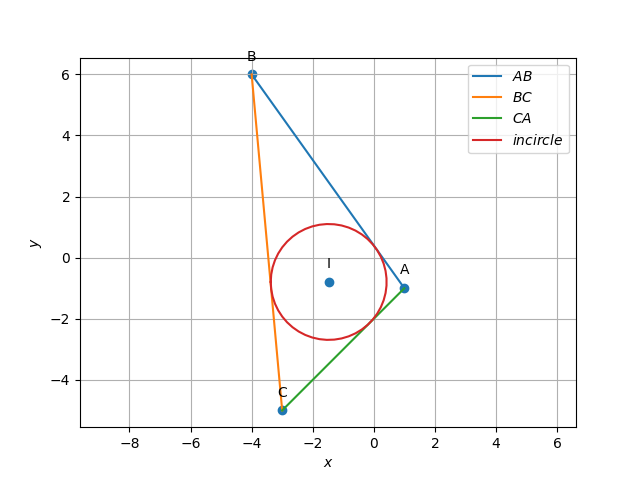
\includegraphics[width=\columnwidth]{solutions/1/5/7/figs/Diagram.png}
	\caption{Triangle with the incircle generated using python}
	\label{fig:Incircle}
\end{figure}

	The equation of the incircle is given as :

	\begin{align}
			\norm{\vec{x}-\vec{I}}^2 = r^2
	\end{align}

	\item Obtain $m,n,p$ in terms of $a,b,c$, the sides of the triangle using a matrix equation.  Obtain the numerical values.
 \\
 		\solution 
From the given information, 
\begin{align}
% 
    a &= m+n,\\
    b &= n+p, \\
    c &= m+p 
\end{align}
which can be expressed as
\begin{align}
\myvec{1&1&0\\0&1&1\\1&0&1\\}\myvec{m\\n\\p} &= \myvec{a\\b\\c}
\\
\implies 
	\myvec{m\\n\\p} &= \myvec{1&1&0\\0&1&1\\1&0&1\\}^{-1}\myvec{a\\b\\c}
\end{align}
Using row reduction,
		\begin{align}
			\augvec{3}{3}{1&1&0 & 1 & 0 & 0\\0&1&1 & 0 & 1 & 0\\1&0&1 & 0 & 0 & 1}
			\xleftrightarrow[]{R_3 \leftarrow R_3 - R_1}
			\augvec{3}{3}{1&1&0 & 1 & 0 & 0\\0&1&1 & 0 & 1 & 0\\0&-1&1 & -1 & 0 & 1}
		\end{align}
		\begin{align}
			\xleftrightarrow[R_1 \leftarrow R_1 - R_2]{R_3 \leftarrow R_3 + R_2}
			\augvec{3}{3}{1&0&-1 & 1 & -1 & 0\\0&1&1 & 0 & 1 & 0\\0&0&2 & -1 & 1 & 1}
		\end{align}
		\begin{align}
			\xleftrightarrow[R_1 \leftarrow 2R_1 + R_3]{R_2 \leftarrow 2R_2 - R_3}
			\augvec{3}{3}{2&0&0 & 1 & -1 & 1\\0&2&0 & 1 & 1 & -1\\0&0&2 & -1 & 1 & 1}
		\end{align}
yielding
		\begin{align}
			\myvec{1&1&0\\0&1&1\\1&0&1\\}^{-1} = 
			\frac{1}{2}\myvec{1 & -1 & 1\\ 1 & 1 & -1\\ -1 & 1 & 1}
		\end{align}
	Therefore,
\begin{align}
\begin{split}
    p&=\frac{c+b-a}{2}
    =\frac{\sqrt{74}+\sqrt{32}-\sqrt{122}}{2}
    \\
    m&=\frac{a+c-b}{2}
    =\frac{\sqrt{74}+\sqrt{122}-\sqrt{32}}{2}
    \\
    n&=\frac{a+b-c}{2}
    =\frac{\sqrt{122}+\sqrt{32}-\sqrt{74}}{2}
\end{split}
	\label{eq:incircle-mnp}
\end{align}
upon substituting from 
		\eqref{eq:geo-norm-ab},
		\eqref{eq:geo-norm-bc}
		and
		\eqref{eq:geo-norm-ca}.

\end{enumerate}
